% Options for packages loaded elsewhere
\PassOptionsToPackage{unicode}{hyperref}
\PassOptionsToPackage{hyphens}{url}
\PassOptionsToPackage{dvipsnames,svgnames,x11names}{xcolor}
%
\documentclass[
  letterpaper,
  DIV=11,
  numbers=noendperiod]{scrartcl}

\usepackage{amsmath,amssymb}
\usepackage{lmodern}
\usepackage{iftex}
\ifPDFTeX
  \usepackage[T1]{fontenc}
  \usepackage[utf8]{inputenc}
  \usepackage{textcomp} % provide euro and other symbols
\else % if luatex or xetex
  \usepackage{unicode-math}
  \defaultfontfeatures{Scale=MatchLowercase}
  \defaultfontfeatures[\rmfamily]{Ligatures=TeX,Scale=1}
\fi
% Use upquote if available, for straight quotes in verbatim environments
\IfFileExists{upquote.sty}{\usepackage{upquote}}{}
\IfFileExists{microtype.sty}{% use microtype if available
  \usepackage[]{microtype}
  \UseMicrotypeSet[protrusion]{basicmath} % disable protrusion for tt fonts
}{}
\makeatletter
\@ifundefined{KOMAClassName}{% if non-KOMA class
  \IfFileExists{parskip.sty}{%
    \usepackage{parskip}
  }{% else
    \setlength{\parindent}{0pt}
    \setlength{\parskip}{6pt plus 2pt minus 1pt}}
}{% if KOMA class
  \KOMAoptions{parskip=half}}
\makeatother
\usepackage{xcolor}
\setlength{\emergencystretch}{3em} % prevent overfull lines
\setcounter{secnumdepth}{5}
% Make \paragraph and \subparagraph free-standing
\ifx\paragraph\undefined\else
  \let\oldparagraph\paragraph
  \renewcommand{\paragraph}[1]{\oldparagraph{#1}\mbox{}}
\fi
\ifx\subparagraph\undefined\else
  \let\oldsubparagraph\subparagraph
  \renewcommand{\subparagraph}[1]{\oldsubparagraph{#1}\mbox{}}
\fi


\providecommand{\tightlist}{%
  \setlength{\itemsep}{0pt}\setlength{\parskip}{0pt}}\usepackage{longtable,booktabs,array}
\usepackage{calc} % for calculating minipage widths
% Correct order of tables after \paragraph or \subparagraph
\usepackage{etoolbox}
\makeatletter
\patchcmd\longtable{\par}{\if@noskipsec\mbox{}\fi\par}{}{}
\makeatother
% Allow footnotes in longtable head/foot
\IfFileExists{footnotehyper.sty}{\usepackage{footnotehyper}}{\usepackage{footnote}}
\makesavenoteenv{longtable}
\usepackage{graphicx}
\makeatletter
\def\maxwidth{\ifdim\Gin@nat@width>\linewidth\linewidth\else\Gin@nat@width\fi}
\def\maxheight{\ifdim\Gin@nat@height>\textheight\textheight\else\Gin@nat@height\fi}
\makeatother
% Scale images if necessary, so that they will not overflow the page
% margins by default, and it is still possible to overwrite the defaults
% using explicit options in \includegraphics[width, height, ...]{}
\setkeys{Gin}{width=\maxwidth,height=\maxheight,keepaspectratio}
% Set default figure placement to htbp
\makeatletter
\def\fps@figure{htbp}
\makeatother
\newlength{\cslhangindent}
\setlength{\cslhangindent}{1.5em}
\newlength{\csllabelwidth}
\setlength{\csllabelwidth}{3em}
\newlength{\cslentryspacingunit} % times entry-spacing
\setlength{\cslentryspacingunit}{\parskip}
\newenvironment{CSLReferences}[2] % #1 hanging-ident, #2 entry spacing
 {% don't indent paragraphs
  \setlength{\parindent}{0pt}
  % turn on hanging indent if param 1 is 1
  \ifodd #1
  \let\oldpar\par
  \def\par{\hangindent=\cslhangindent\oldpar}
  \fi
  % set entry spacing
  \setlength{\parskip}{#2\cslentryspacingunit}
 }%
 {}
\usepackage{calc}
\newcommand{\CSLBlock}[1]{#1\hfill\break}
\newcommand{\CSLLeftMargin}[1]{\parbox[t]{\csllabelwidth}{#1}}
\newcommand{\CSLRightInline}[1]{\parbox[t]{\linewidth - \csllabelwidth}{#1}\break}
\newcommand{\CSLIndent}[1]{\hspace{\cslhangindent}#1}

\KOMAoption{captions}{tableheading}
\makeatletter
\makeatother
\makeatletter
\makeatother
\makeatletter
\@ifpackageloaded{caption}{}{\usepackage{caption}}
\AtBeginDocument{%
\ifdefined\contentsname
  \renewcommand*\contentsname{Table of contents}
\else
  \newcommand\contentsname{Table of contents}
\fi
\ifdefined\listfigurename
  \renewcommand*\listfigurename{List of Figures}
\else
  \newcommand\listfigurename{List of Figures}
\fi
\ifdefined\listtablename
  \renewcommand*\listtablename{List of Tables}
\else
  \newcommand\listtablename{List of Tables}
\fi
\ifdefined\figurename
  \renewcommand*\figurename{Figure}
\else
  \newcommand\figurename{Figure}
\fi
\ifdefined\tablename
  \renewcommand*\tablename{Table}
\else
  \newcommand\tablename{Table}
\fi
}
\@ifpackageloaded{float}{}{\usepackage{float}}
\floatstyle{ruled}
\@ifundefined{c@chapter}{\newfloat{codelisting}{h}{lop}}{\newfloat{codelisting}{h}{lop}[chapter]}
\floatname{codelisting}{Listing}
\newcommand*\listoflistings{\listof{codelisting}{List of Listings}}
\makeatother
\makeatletter
\@ifpackageloaded{caption}{}{\usepackage{caption}}
\@ifpackageloaded{subcaption}{}{\usepackage{subcaption}}
\makeatother
\makeatletter
\@ifpackageloaded{tcolorbox}{}{\usepackage[many]{tcolorbox}}
\makeatother
\makeatletter
\@ifundefined{shadecolor}{\definecolor{shadecolor}{rgb}{.97, .97, .97}}
\makeatother
\makeatletter
\makeatother
\ifLuaTeX
  \usepackage{selnolig}  % disable illegal ligatures
\fi
\IfFileExists{bookmark.sty}{\usepackage{bookmark}}{\usepackage{hyperref}}
\IfFileExists{xurl.sty}{\usepackage{xurl}}{} % add URL line breaks if available
\urlstyle{same} % disable monospaced font for URLs
\hypersetup{
  pdftitle={Analysis of Customer Complaints on US Financial Products},
  pdfauthor={Ty Andrews; Dhruvi Nishar; Luke Yang},
  colorlinks=true,
  linkcolor={blue},
  filecolor={Maroon},
  citecolor={Blue},
  urlcolor={Blue},
  pdfcreator={LaTeX via pandoc}}

\title{Analysis of Customer Complaints on US Financial Products}
\author{Ty Andrews \and Dhruvi Nishar \and Luke Yang}
\date{}

\begin{document}
\maketitle
\ifdefined\Shaded\renewenvironment{Shaded}{\begin{tcolorbox}[borderline west={3pt}{0pt}{shadecolor}, interior hidden, sharp corners, enhanced, breakable, frame hidden, boxrule=0pt]}{\end{tcolorbox}}\fi

\renewcommand*\contentsname{Table of contents}
{
\hypersetup{linkcolor=}
\setcounter{tocdepth}{3}
\tableofcontents
}
\hypertarget{summary}{%
\section{Summary}\label{summary}}

Here we used multiple classification algorithms to predict whether a
financial product consumer will dispute a complaint made to the Consumer
Financial Protection Bureaus' (CFPB) Consumer Complaints
Database(\emph{Consumer Complaints Database} 2022).

\hypertarget{introduction}{%
\section{Introduction}\label{introduction}}

As of 2022, the CFPB receives over 60,000 consumer complaints a month
related to companies financial products. Between December 2011 and
November 2022 over 140,000 complaints were disputed by consumers costing
both the companies and CFPB time and money.

\hypertarget{methods}{%
\section{Methods}\label{methods}}

\hypertarget{data}{%
\subsection{Data}\label{data}}

Complaints can be responded to by the company in multiple ways but each
consumer has the opportunity to dispute the provided response. These
disputes are likely costly to both the CFPB and the companies for which
they are raised so being able to anticipate whether a complaint will be
disputed has the potential to save both time and money for companies and
the CFPB alike.

\begin{figure}

{\centering 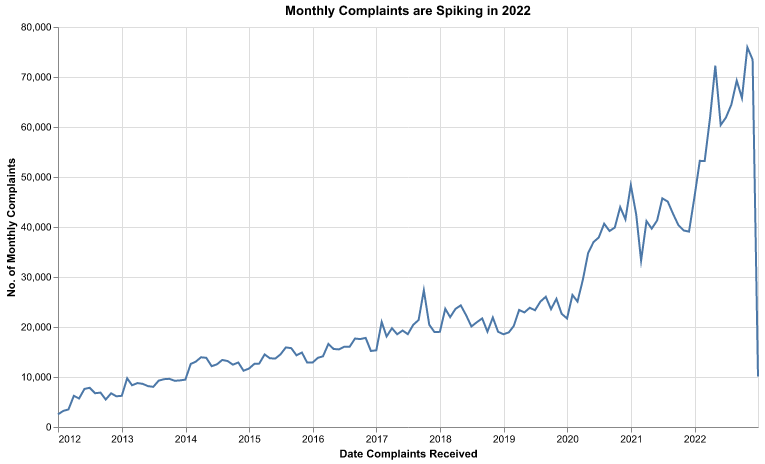
\includegraphics{assets/complaints_over_time_line.png}

}

\caption{Figure 1. Monthly complaints since 2012.}

\end{figure}

The CFPB database contains \textasciitilde3 million complaints starting
from December 2011 all the way up to November 2022 when this report was
written. Approximately 4.8\% of all complaints are disputed, with the
\textasciitilde75.1\% of complaints having an unknown dispute status.
Figure 2 below shows the balance of dispute status.

\begin{figure}

{\centering 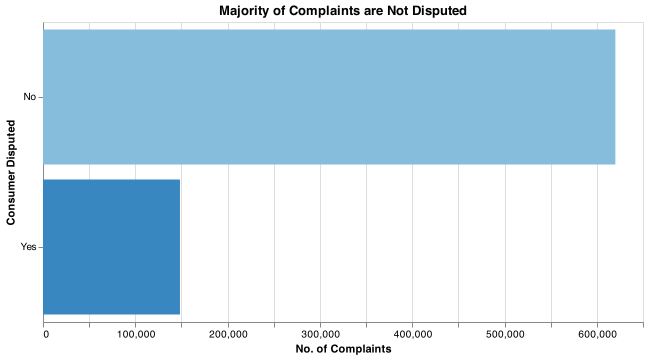
\includegraphics{assets/disputed_bar.png}

}

\caption{Figure 2. Class Imbalance in the Target Column}

\end{figure}

Each field has varying amounts of missing values as can be seen in Table
1 below. Fields such as tag where there are numerous entries missing
values were removed from the analysis. Individual complaints with
missing information were removed from the data-set for analysis since
the data set is large enough to still have a significant number of
training examples for the analysis (\textasciitilde20,000).

\begin{longtable}[]{@{}lcc@{}}
\caption{Table 1. Unique and missing value counts by data
feature.}\tabularnewline
\toprule()
Fields & Valid Count & Unique Count \\
\midrule()
\endfirsthead
\toprule()
Fields & Valid Count & Unique Count \\
\midrule()
\endhead
date\_received & 3084450 & 4003 \\
product & 3084450 & 18 \\
sub\_product & 2849156 & 76 \\
issue & 3084450 & 165 \\
sub\_issue & 2401899 & 221 \\
consumer\_complaint\_narrative & 1107253 & 967541 \\
company\_public\_response & 1339720 & 11 \\
company & 3084450 & 6565 \\
state & 3044459 & 63 \\
zip\_code & 3043948 & 34429 \\
tags & 350065 & 3 \\
consumer\_consent\_provided & 2264772 & 4 \\
submitted\_via & 3084450 & 7 \\
date\_sent\_to\_company & 3084450 & 3952 \\
company\_response\_to\_consumer & 3084446 & 8 \\
timely\_response & 3084450 & 2 \\
consumer\_disputed & 768443 & 2 \\
complaint\_id & 3084450 & 3084450 \\
\bottomrule()
\end{longtable}

\hypertarget{analysis}{%
\subsection{Analysis}\label{analysis}}

A predictive approach using multiple classification models was used to
attempt to predict whether a consumer would dispute a complaint or not.

Feature pre-processing approach and rationale is as follows:

Table 2: Feature selection and encodings.

\begin{longtable}[]{@{}
  >{\raggedright\arraybackslash}p{(\columnwidth - 4\tabcolsep) * \real{0.3163}}
  >{\raggedright\arraybackslash}p{(\columnwidth - 4\tabcolsep) * \real{0.2245}}
  >{\raggedright\arraybackslash}p{(\columnwidth - 4\tabcolsep) * \real{0.4592}}@{}}
\caption{These features were passed into a column transformer, which was
then integrated with five different estimator for
prediction.}\tabularnewline
\toprule()
\begin{minipage}[b]{\linewidth}\raggedright
Features
\end{minipage} & \begin{minipage}[b]{\linewidth}\raggedright
Preprocessing Step
\end{minipage} & \begin{minipage}[b]{\linewidth}\raggedright
Rationale
\end{minipage} \\
\midrule()
\endfirsthead
\toprule()
\begin{minipage}[b]{\linewidth}\raggedright
Features
\end{minipage} & \begin{minipage}[b]{\linewidth}\raggedright
Preprocessing Step
\end{minipage} & \begin{minipage}[b]{\linewidth}\raggedright
Rationale
\end{minipage} \\
\midrule()
\endhead
consumer\_complaint\_narrative & CountVectorizer

max\_features = 1000 & High Amount of Unique Textual Data \\
product

sub\_product

issue

company\_public\_response

company

company\_response\_to\_consumer & OneHotEncoder

drop = ``if\_binary'' & Each field is categorical \\
consumer\_consent\_provided & dropped & Single Category \\
\bottomrule()
\end{longtable}

\hypertarget{results-discussion}{%
\section{Results \& Discussion}\label{results-discussion}}

We applied the \texttt{DummyClassifier}, \texttt{LogisticRegression},
\texttt{Naive\ Bayes}, \texttt{SVC}, and \texttt{RandomForestClassifier}
to predict the target whether the customer disputed. The models were
applied using default parameters and a five-fold cross-validation were
applied using the training split. We examined and recorded the accuracy,
precision, recall, and f1 scores to be the metrics evaluating the
models. The results of the cross validation were as follows:

\begin{longtable}[]{@{}
  >{\centering\arraybackslash}p{(\columnwidth - 10\tabcolsep) * \real{0.1951}}
  >{\centering\arraybackslash}p{(\columnwidth - 10\tabcolsep) * \real{0.0854}}
  >{\centering\arraybackslash}p{(\columnwidth - 10\tabcolsep) * \real{0.2561}}
  >{\centering\arraybackslash}p{(\columnwidth - 10\tabcolsep) * \real{0.1585}}
  >{\centering\arraybackslash}p{(\columnwidth - 10\tabcolsep) * \real{0.1098}}
  >{\centering\arraybackslash}p{(\columnwidth - 10\tabcolsep) * \real{0.1951}}@{}}
\caption{Table 3. Model Performance and Score.}\tabularnewline
\toprule()
\begin{minipage}[b]{\linewidth}\centering
Metric
\end{minipage} & \begin{minipage}[b]{\linewidth}\centering
Dummy
\end{minipage} & \begin{minipage}[b]{\linewidth}\centering
Logistic Regression
\end{minipage} & \begin{minipage}[b]{\linewidth}\centering
Naive Bayes
\end{minipage} & \begin{minipage}[b]{\linewidth}\centering
SVC
\end{minipage} & \begin{minipage}[b]{\linewidth}\centering
Random Forest
\end{minipage} \\
\midrule()
\endfirsthead
\toprule()
\begin{minipage}[b]{\linewidth}\centering
Metric
\end{minipage} & \begin{minipage}[b]{\linewidth}\centering
Dummy
\end{minipage} & \begin{minipage}[b]{\linewidth}\centering
Logistic Regression
\end{minipage} & \begin{minipage}[b]{\linewidth}\centering
Naive Bayes
\end{minipage} & \begin{minipage}[b]{\linewidth}\centering
SVC
\end{minipage} & \begin{minipage}[b]{\linewidth}\centering
Random Forest
\end{minipage} \\
\midrule()
\endhead
fit\_time & 0.978 & 5.475 & 1.674 & 123.556 & 22.726 \\
score\_time & 0.257 & 0.431 & 0.369 & 24.588 & 0.592 \\
test\_accuracy & 0.779 & 0.655 & 0.702 & 0.679 & 0.784 \\
test\_recall & 0.000 & 0.455 & 0.342 & 0.445 & 0.056 \\
test\_precision & 0.000 & 0.309 & 0.332 & 0.331 & 0.631 \\
test\_f1 & 0.000 & 0.368 & 0.337 & 0.380 & 0.102 \\
\bottomrule()
\end{longtable}

Figure 3 below illustrates a visual representation of the performance of
the models. We observe a high accuracy of the \texttt{DummyClassifier}.
Given the imbalance of the class, the accuracy would not be an important
metric in this problem. Instead, from the company's perspective, we
focus more on improving the precision, the recall, and the f1 score.
Noticeably the company likely wants to spot the people who are going to
dispute, thus, the recall score here is more important compared to
precision.

\begin{figure}

{\centering 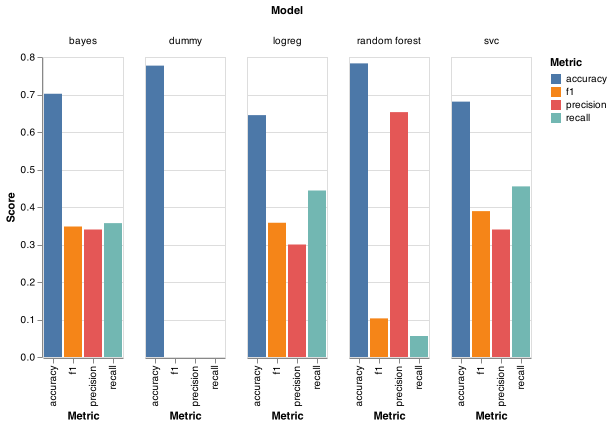
\includegraphics{assets/model_performance.png}

}

\caption{Figure 3: Performance of Different Models on Different Metrics}

\end{figure}

The results above motivates us to choose \texttt{LogisticRegression} as
the final estimator. It has one of the overall highest f1 scores at
0.368 and among the recall is among highest scores. Though it sacrifices
some accuracy, the precision, recall, and f1 scores are significantly
improved uon the dummy classifier and competitive with the other models
evaluated. We also see that \texttt{SVC} gives slightly higher scores
than \texttt{LogisticRegression}; however, in Table 2 we see that it
takes substantially more time to train and cross validate. in addition,
due to the complexity of the model we also lose a degree of model
incontestability. Overall, we choose \texttt{LogisticRegression} over
\texttt{SVC} due to its scalability and interpretability.

Unfortunately, an f1 score of 0.368 for \texttt{LogisticRegression} is
quite low and unlikely to be particularly useful in the broader business
sense. This analysis can be used as the basis to understand what target
f1, precision or recall target scores should be set for further
analysis.

\hypertarget{conclusion}{%
\section{Conclusion}\label{conclusion}}

The analysis in this reports focuses on using a machine learning
approach to predict whether the consumer is going to dispute after the
company's response. We processed the features such as the product,
consumer's complaints, and company's responses. We trained five
different models that optimized the f1 score and chose
\texttt{LogisticRegression} as a suitable estimator for the first pass
at attempting to predict whether consumers dispute their complaints.
Next steps would be evaluating the impact of the chosen models
performance and then deciding whether to try and refine further to
improve the model.

\hypertarget{references}{%
\section*{References}\label{references}}
\addcontentsline{toc}{section}{References}

\hypertarget{refs}{}
\begin{CSLReferences}{1}{0}
\leavevmode\vadjust pre{\hypertarget{ref-COMPL_DB}{}}%
\emph{Consumer Complaints Database}. 2022. Consumer Financial Protection
Bureau.
\url{https://www.consumerfinance.gov/data-research/consumer-complaints/\#download-the-data}.

\end{CSLReferences}



\end{document}
